\documentclass[nooutcomes]{ximera}
%% handout
%% space
%% newpage
%% numbers
%% nooutcomes

%I added the commands here so that I would't have to keep looking them up
%\newcommand{\RR}{\mathbb R}
%\renewcommand{\d}{\,d}
%\newcommand{\dd}[2][]{\frac{d #1}{d #2}}
%\renewcommand{\l}{\ell}
%\newcommand{\ddx}{\frac{d}{dx}}
%\everymath{\displaystyle}
%\newcommand{\dfn}{\textbf}
%\newcommand{\eval}[1]{\bigg[ #1 \bigg]}

%\begin{image}
%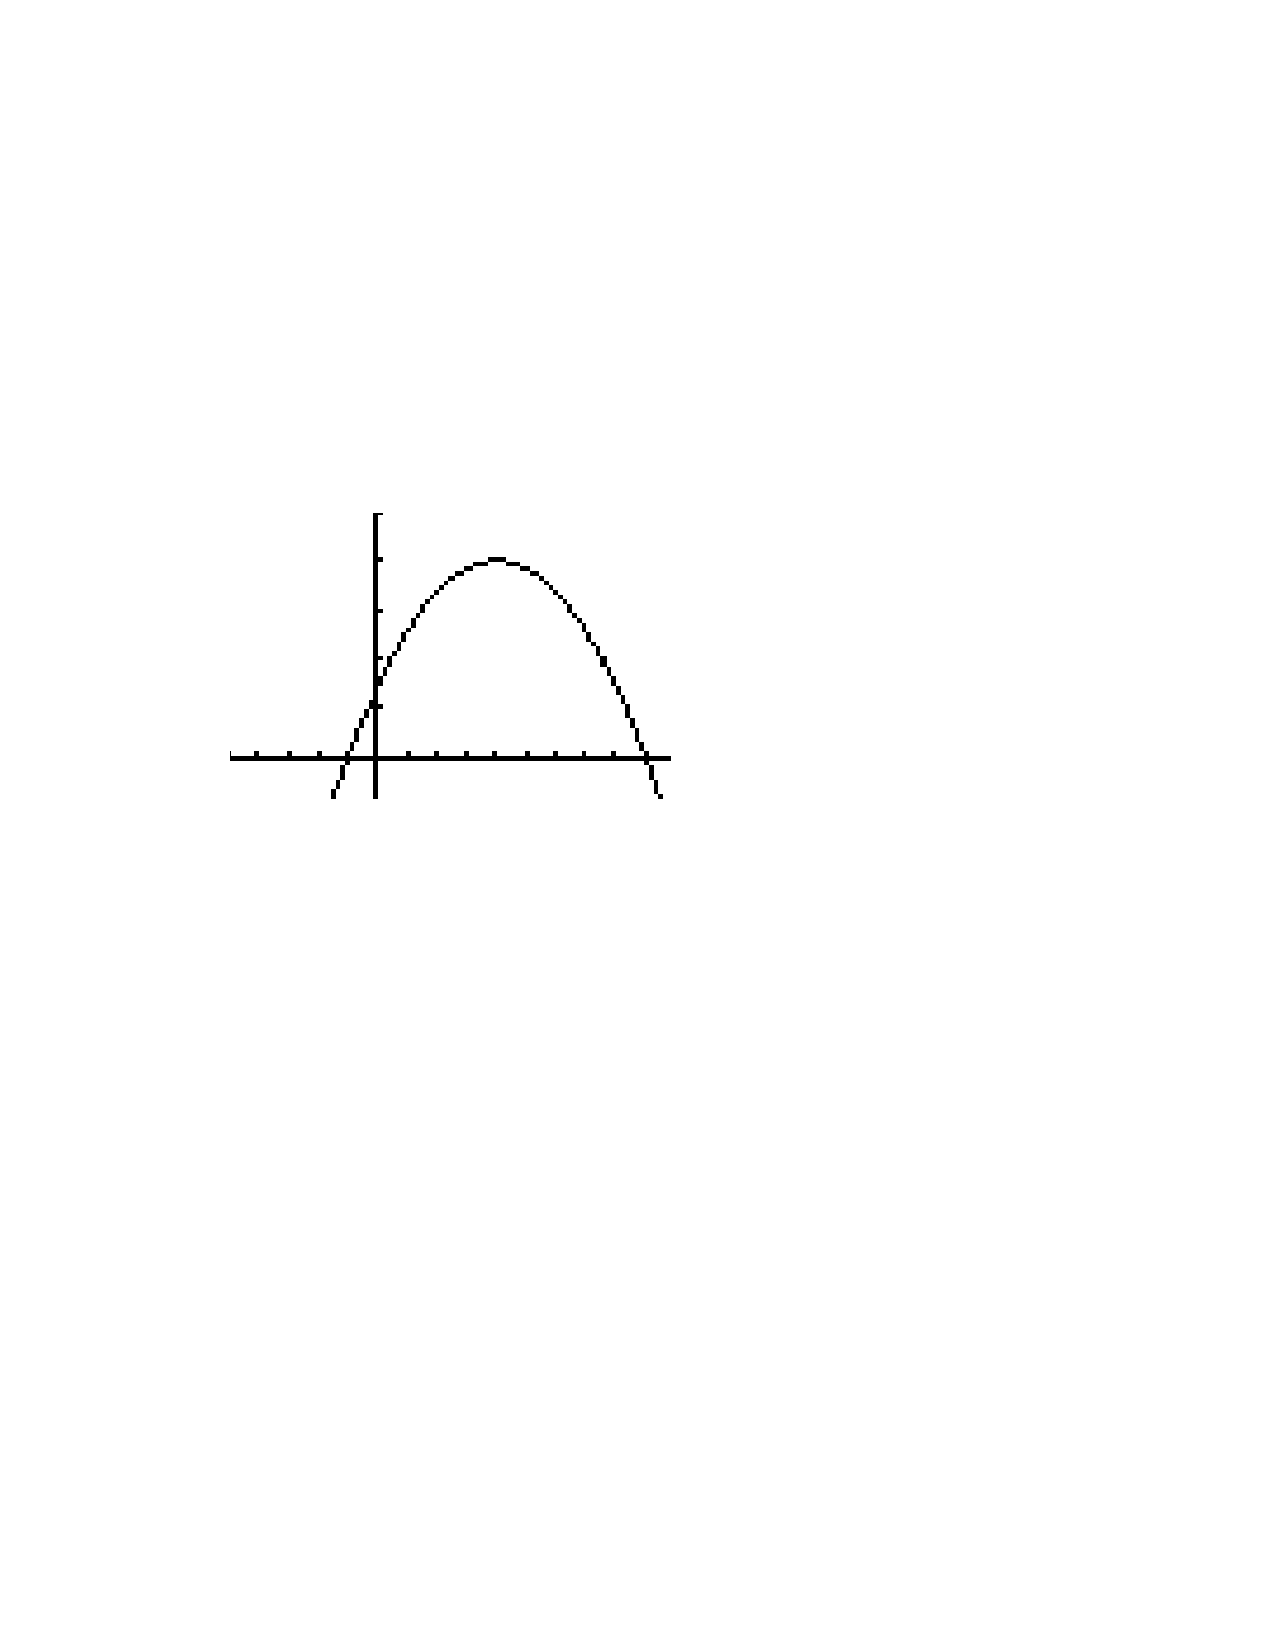
\includegraphics[trim= 170 420 250 180]{Figure1.pdf}
%\end{image}


\newcommand{\RR}{\mathbb R}
\renewcommand{\d}{\,d}
\newcommand{\dd}[2][]{\frac{d #1}{d #2}}
\renewcommand{\l}{\ell}
\newcommand{\ddx}{\frac{d}{dx}}
\newcommand{\dfn}{\textbf}
\newcommand{\eval}[1]{\bigg[ #1 \bigg]}

\usepackage{multicol}

\renewenvironment{freeResponse}{
\ifhandout\setbox0\vbox\bgroup\else
\begin{trivlist}\item[\hskip \labelsep\bfseries Solution:\hspace{2ex}]
\fi}
{\ifhandout\egroup\else
\end{trivlist}
\fi} %% we can turn off input when making a master document

\title{3.9 Derivatives of Logarithmic and Exponential Functions (Solutions)}  

\begin{document}
\begin{abstract}		\end{abstract}
\maketitle

\section*{Warm up:} 
	\begin{enumerate}
	
	%part 1
	\item[(1)]  If $f(x) = (x-2)^x$, then $f'(x) = x (x-2)^{x-1}$.

		\begin{freeResponse}
		False.  Any time that you have a function of $x$ raised to a function of $x$, in order to compute the derivative you need to use logarithmic differentiation (or something equivalent).
		\end{freeResponse}	
		
		
		
	%part 2
	\item[(2)]  If $f(x) = (3x)^x$, then $f'(x) = (3x)^x \ln (3x)$.

		\begin{freeResponse}
		False.  Same as part (1).  
		\end{freeResponse}	
		
		
		
	\end{enumerate}
		
		
		

	
	
	
	
	

\section*{Group work:}



%problem 1
\begin{problem}
Find the derivatives of the following functions:
	\begin{enumerate}
	
	%part a
	\item  $f(x) = x^{e^x} + 7x$
		\begin{freeResponse}
		$f'(x) = \ddx \left(x^{e^x} \right) + \ddx(7x) = \ddx \left(x^{e^x} \right) + 7$.  So the real problem is to find $\ddx \left(x^{e^x} \right)$.  
		
		\begin{align*}
		\ddx \left( x^{e^x} \right) &= \ddx \left( e^{\ln x^{e^x}} \right) \\
		&= \ddx \left( e^{e^x \ln x} \right) \\
		&= e^{e^x \ln x} \left( e^x \ln x + \frac{e^x}{x} \right) \\
		&= x^{e^x} \left( e^x \ln x + \frac{e^x}{x} \right).
		\end{align*}
		
		Thus, $f'(x) = x^{e^x} \left( e^x \ln x + \frac{e^x}{x} \right) + 7$.  
		
		\end{freeResponse}
		
		
		
	%part b
	\item  $g(x) = (\ln x + 9)^{\sec(x^4)}$
		\begin{freeResponse}
			\begin{align*}
			g'(x) &= \ddx \left( (\ln x + 9)^{\sec(x^4)} \right) \\
			&= \ddx \left( e^{\sec(x^4) \ln ( \ln x + 9) } \right) \\
			&= e^{\sec(x^4) \ln ( \ln x + 9)} \left( 4x^3 \sec(x^4) \tan(x^4) \ln(\ln x + 9) + \sec(x^4) \frac{\frac{1}{x}}{\ln x + 9} \right) \\
			&= (\ln x + 9)^{\sec(x^4)} \left( 4x^3 \sec(x^4) \tan(x^4) \ln(\ln x + 9) + \frac{\sec(x^4)}{x(\ln x + 9)} \right) .
			\end{align*}
		\end{freeResponse}
		
		
		
	%part c
	\item  $h(x) = \sqrt[4]{\frac{(x^2 - 7)^5 \ln x}{\cos^7(x^2 - 5)}}$
		\begin{freeResponse}
		$$h'(x) = \ddx \left( \left( \frac{(x^2 - 7)^5 \ln x}{\cos^7(x^2 - 5)} \right)^{\frac{1}{4}} \right) $$
		
		$$=  \frac{1}{4} \left( \frac{(x^2 - 7)^5 \ln x}{\cos^7(x^2 - 5)} \right)^{\frac{-3}{4}} \cdot $$
		$$\left( \frac{\cos^7(x^2 - 5)(5(x^2-7)^4(2x) \ln x + (x^2-7)^5 \frac{1}{x}) - (x^2-7)^5 \ln x (7\cos^6(x^2-5) (-\sin(x^2 - 5))(2x))}{\cos^{14}(x^2 - 5)} \right)$$
		\end{freeResponse}
		
		
		
	\end{enumerate}
		
		
\end{problem}
















%problem 2
\begin{problem}

		\begin{freeResponse}
		
		\end{freeResponse}
		
		
		

\end{problem}
	
	
	
	
	
	
	
	
			
			

%problem 3
\begin{problem}

		\begin{freeResponse}
			
		\end{freeResponse}
			
			
		
\end{problem}











%problem 4
\begin{problem}

		\begin{freeResponse}

		\end{freeResponse}
			
			
	
\end{problem}






	
	
	
	
	
	
	
	
	

	










								
				
				
	














\end{document} 


















